\subsection{Lower research productivity}
\label{subsec:rewrite-rsi-research-share}

I now set $\chi=1.5$, one fifth of its value in
Section~\ref{subsec:rewrite-rsi-half-decline}. All other parameters and
initial stocks remain unchanged, including the elasticity-specific
pre-RSI capital stocks in Table~\ref{tab:rewrite-rsi-parameters}.
Consumption and research are solved again for each economy; the new
exercise changes both the initial adjustment and the timing of the
transition, but not the limiting growth rates, interest rates, and income shares.

% The generated numerical digest in rsi_chi_1_5_results.tex is retained,
% but not input here: editorial prose is organized around the three figures.
% Source: numerical_rewrite/rsi_chi_1_5/{summary,figure_manifest}.json.
I use Figure~\ref{fig:rewrite-rsi-research-accumulation} to present the growth of $Y/(AL)$, $X/(AL)$, and $K/(AL)$ in panels A--C, in percent
per year. As before, zero means growth at the rate of effective labor, $n+\gamma$. The upper row shows two pre-event years and the first ten years after RSI activation. The lower row follows the same trajectories
from year 10 to year 500. Throughout the three figures, line styles identify the same four elasticities as in Figure~\ref{fig:rewrite-rsi-half-accumulation}, and black dotted lines mark the analytical limits for $\sigma=1.50$. %Vertical scales differ between exercises.

\begin{figure}[H]
 \centering
 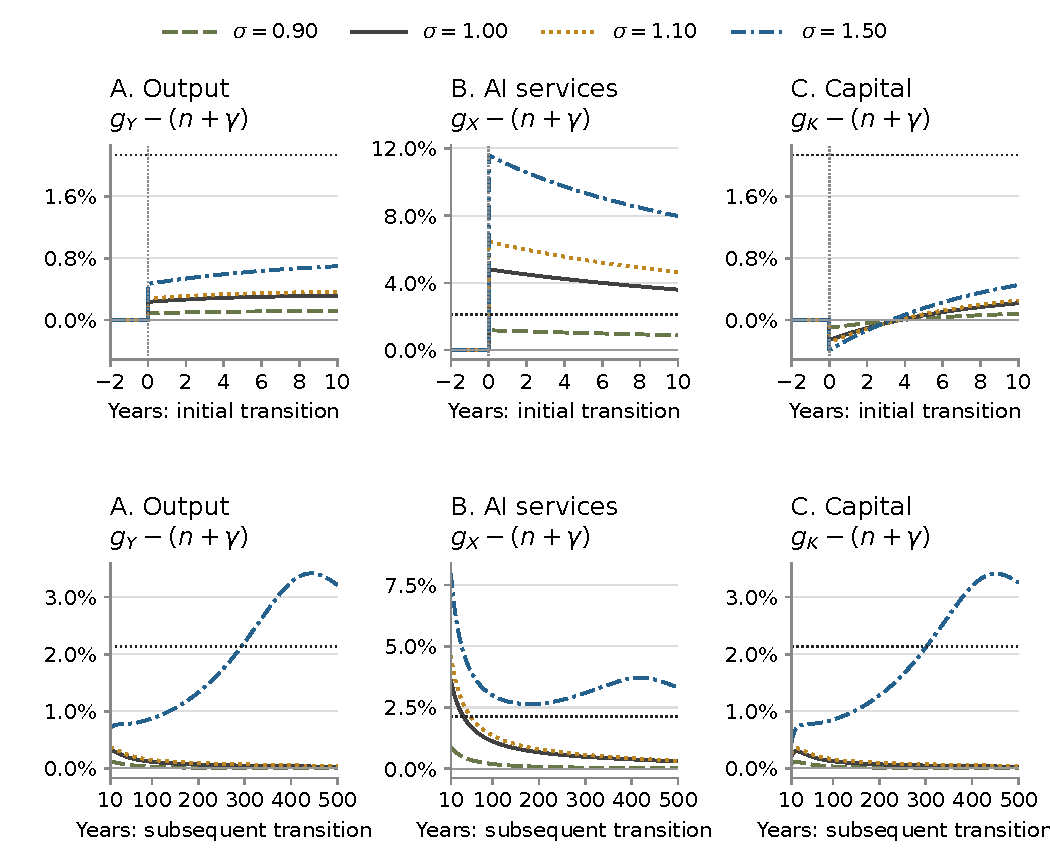
\includegraphics[width=\textwidth]{figures_rewrite/equilibrium_rsi_chi_1_5_accumulation_growth_windows.pdf}
 \caption{Lower research productivity ($\chi=1.5$): growth of output,
 AI production services, and capital per unit of effective labor.
 Rates are instantaneous annual rates. The upper row shows two pre-event
 years and years 0--10; the lower row shows years 10--500. Panels A and C
 share a scale within each row. The vertical line marks RSI activation.}
 \label{fig:rewrite-rsi-research-accumulation}
\end{figure}

The upper row shows a much smaller initial increase in growth.
Growth of $Y/(AL)$ ranges from $0.1\%$ to $0.5\%$ across the four
economies. AI services still grow faster than output, but their initial
normalized growth rate at $\sigma=1.50$ is $11.6\%$, compared with
$80.8\%$ in the preceding exercise. Lower research productivity and a
smaller research allocation produce slower efficiency improvements.
Consumption still rises at activation, and research uses resources that
could otherwise finance capital accumulation. Both adjustments are
smaller, however, so $K/(AL)$ falls less. As capital accumulation
recovers, output growth rises during the first decade even though
AI-service growth is already slowing. The four economies therefore
begin with more moderate growth and less pronounced differences.

The lower row reveals the eventual separation between regimes. At $\sigma=1.50$, output and capital growth rise for several centuries before declining. AI-service growth first slows, then rises again as capital and inference use expand. At year 500, $Y/(AL)$ still grows at $3.2\%$, above its $2.1\%$ long-run limit, showing a significantly slower transition.
A similar pattern of delayed acceleration appears in
\citet[pp.~11--12]{jones2026future}, drawing on
\citet{jonestonetti2026}. My simulations generate the transition
through private RSI investment and capital accumulation, without
modeling the progressive automation of additional tasks.
%Proposition~\ref{prop:rewrite-equilibrium-regimes} gives the same limits in both exercises of section \ref{subsec:rewrite-rsi-activation} and \ref{subsec:rewrite-rsi-half-decline}: output and capital growth rates tends to the effective labor growth rate in the three labor-bottleneck cases and remains above it at $\sigma=1.50$.

I next examine wages and prices in Figure~\ref{fig:rewrite-rsi-research-prices}. Panels A--C show annual wage growth $g_w$, the annual net interest rate $r$, and the level of $p_X$ in final-good units on a logarithmic scale. The top panels show the short run and the bottom panels the long run. Initially, wage growth rises modestly in all four economies. Unlike the preceding exercise, it continues to increase during the first years even in the labor-bottleneck cases: capital accumulation helps sustain the increase in labor's marginal product. The interest rate also rises more gradually as output outpaces capital. At $\sigma=1.50$, it reaches $5.5\%$ after ten years, compared with $7.8\%$ under higher research productivity. Meanwhile, slower efficiency improvements make the decline in $p_X$ more gradual.

In the bottom row, wage growth and the interest rate eventually turn down in all four economies. The three labor-bottleneck cases approach $1.0\%$ and $5.0\%$, respectively. At $\sigma=1.50$, the rise and
subsequent decline occur much later, and adjustment remains incomplete at year 500: the interest rate is still $8.2\%$, above its $7.1\%$
long-run value. The limiting wage-growth rate remains $2.4\%$, below output-per-worker growth of $3.1\%$. Lower research productivity therefore delays the transition without eliminating the long-run difference between these growth rates. %At year 500, the AI-service price in this case is already close to its positive limit, even though growth and interest rates are still adjusting.

\begin{figure}[H]
 \centering
 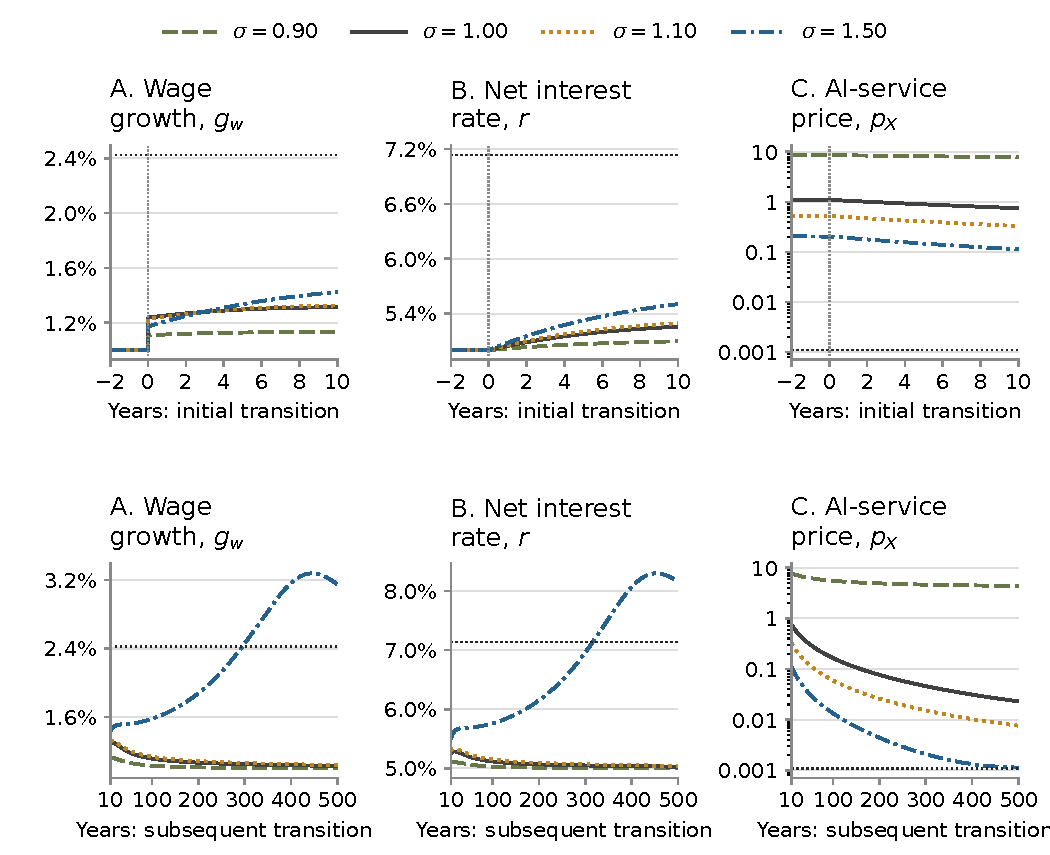
\includegraphics[width=\textwidth]{figures_rewrite/equilibrium_rsi_chi_1_5_growth_returns_windows.pdf}
 \caption{Lower research productivity ($\chi=1.5$): wage growth,
 the net interest rate, and the AI-service price. Rates are annual;
 the price is in final-good units on a logarithmic scale.
 The vertical line marks RSI activation.}
 \label{fig:rewrite-rsi-research-prices}
\end{figure}

I complete the comparison with Figure~\ref{fig:rewrite-rsi-research-distribution}. Panels A--D report
$wL/Y$, $\Pi/Y$, $U/Y$, and $M/Y$, all as percentages of output. The upper two rows cover the initial transition and the lower two cover years 10--500, with the same scenario lines. The omitted gross capital share remains $33.0\%$.

\begin{figure}[H]
 \centering
 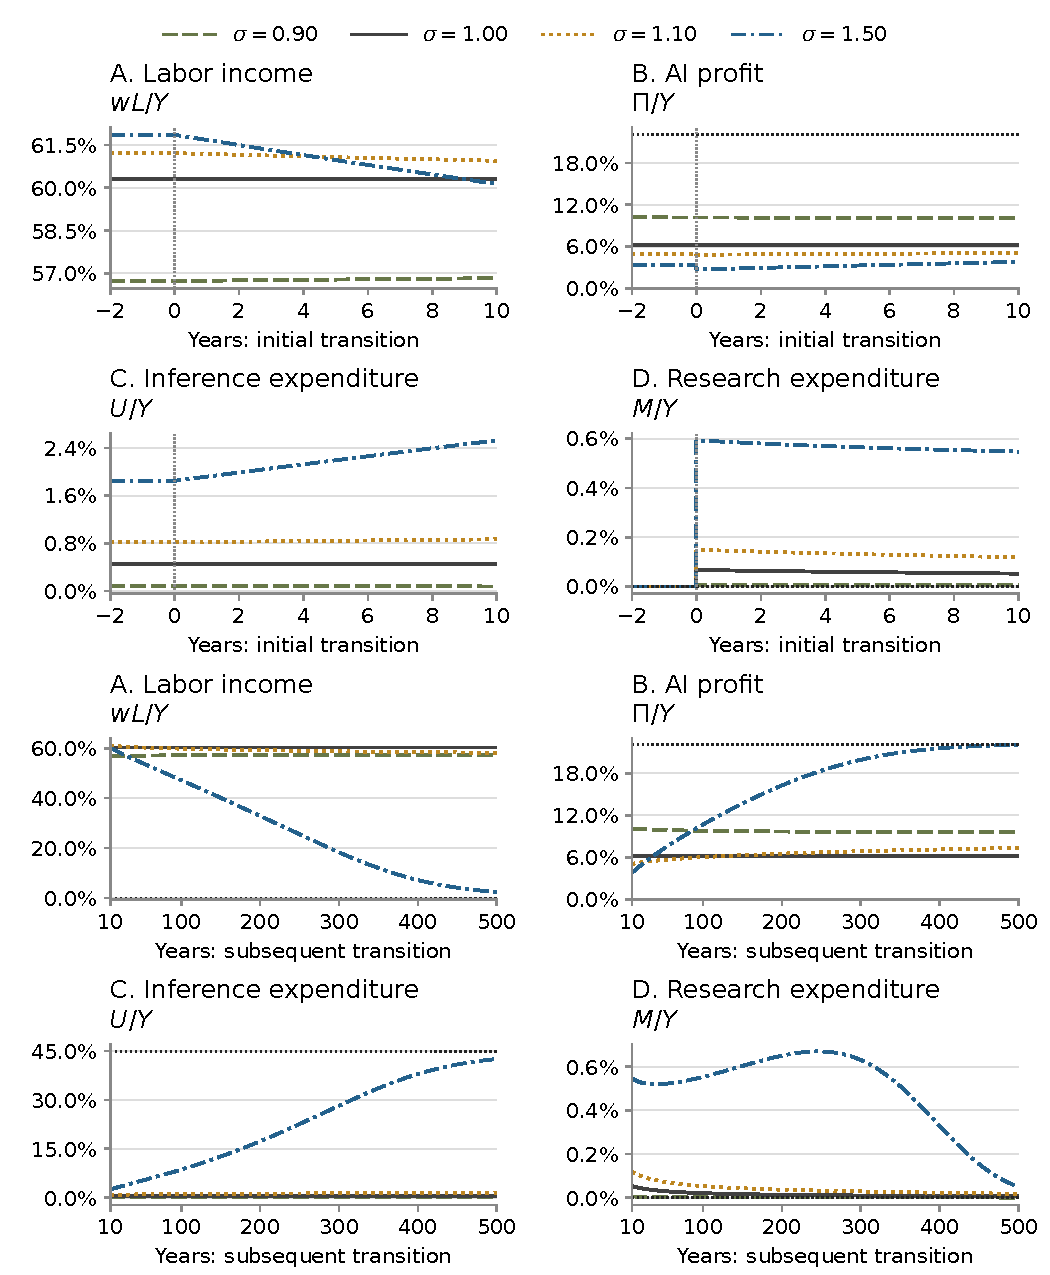
\includegraphics[width=\textwidth]{figures_rewrite/equilibrium_rsi_chi_1_5_ai_distribution_windows.pdf}
 \caption{Lower research productivity ($\chi=1.5$): labor income,
 AI net profit, inference expenditure, and research expenditure relative
 to output. The first two rows show the pre-event BGP and years 0--10;
 the last two show years 10--500. The omitted gross capital share
 remains $\alpha=0.33$. Short-run panels A and C use scales fitted to the
 initial trajectories and omit the long-run reference lines.}
 \label{fig:rewrite-rsi-research-distribution}
\end{figure}

In the short run, research absorbs a smaller share of output, leaving more of AI revenue as net profit. At $\sigma=1.50$, initial research expenditure is $0.6\%$ of output rather than $3.1\%$, and net profit is $2.7\%$ rather than $0.2\%$. Research spending reduces net profit at activation, but less sharply than in the preceding exercise. Inference expenditure and labor's income share change little in the labor-bottleneck cases. In the AI-dominated case, inference's share increases and labor's share declines, but both movements are initially gradual, consistent with the smaller output--wage growth gap.

The longer horizon shows the same eventual redistribution as in Figure~\ref{fig:rewrite-rsi-half-distribution}: labor's share tends to zero at $\sigma=1.50$, while inference expenditure and developer profit approach the same positive shares of output. Research expenditure relative to output first declines, then rises again before falling toward zero. Expanding AI sales provide an incentive for further research, while proximity to the upper bound eventually limits the efficiency gains it can deliver. %The research condition~\eqref{eq:rewrite-research-foc} balances these changing benefits against the cost of compute; $\chi$ alone does not determine the research path.
The other three economies retain a positive labor share. Lower research productivity changes the adjustment and delays the divergence between regimes without changing their limiting growth rates and income shares.
